\chapter{Numerical Results}
\label{chap:results}

In this chapter we present a series of convergence and preconditioning experiments. The principle aim is to check the scalability performance of the preconditioned iterative methods for the MHD problem and the two decoupling schemes proposed in Chapter \ref{chap:precond}. All numerical experiments have been carried out in the Python programming language.

\section{Software}

Due to the complex nature of the MHD problem, a number of different libraries have been used both to discretise and then to solve the resulting systems.

The finite element software that was used to discretise \eqref{eq:mhd} was FEniCS \cite{wells2012automated}. The core libraries used within \fenics are DOLFIN \cite{LoggWells2010a,LoggWellsEtAl2012a} the problem-solving interface, FFC \cite{KirbyLogg2006a,LoggOlgaardEtAl2012a,OlgaardWells2010b} the compiler for finite element variational forms, FIAT \cite{Kirby2012a,Kirby2004a} the finite element  tabulator, Instant the just-in-time compiler, UFC \cite{AlnaesLoggEtAl2009a,AlnaesLoggEtAl2012a} the code generator and UFL \cite{AlnaesEtAl2012,Alnaes2012a} the form language.

Along with \fenics we have used a number of purely linear algebra libraries. The main one that has been used is PETSc4PY which is the python interface for PETSc \cite{petsc-web-page,petsc-user-ref}. PETSc has been used mainly for the iterative solvers as well as the blockwise preconditioning setup. The following packages were used to solve the precondition system: HYPRE \cite{falgout2002hypre} as a multigrid solver and for the sparse direct solvers we use UMFPACK \cite{Davis:2004:CPS:992200.992205,Davis:2004:AUV:992200.992206,Davis:1999:CUM:305658.287640,davis1997unsymmetric}, PASTIX \cite{henon2002pastix}, SuperLU \cite{superlu_ug99,li05} and MUMPS \cite{amestoy2000multifrontal,amestoy2001fully,amestoy2006hybrid}.

\section{Problem setup}

When numerically solving a set of linear or non-linear equations the problem needs to be initialised. By this we mean the mesh sequence, non-linear iteration stopping criteria and initial guess setup needs to be defined. In this small section we will briefly cover these aspects.

\paragraph{Mesh sequence} ~\\

To test the performance of both the preconditioners from  chapter \ref{chap:precond} and to validate the code produced by \fenics a sequence of meshes are required. Verifying the code  produces the correct convergence rates, we consider levels, $l$, of uniform grids. The levels define the number of edges between the nodes along the boundary edge to be  $2^l$. For example, consider the third level, $l = 3$, hence the grid generated is the $8\times 8$ grid given in figure \ref{fig:2Dmesh}.
\begin{figure}[h!]
  \centering
    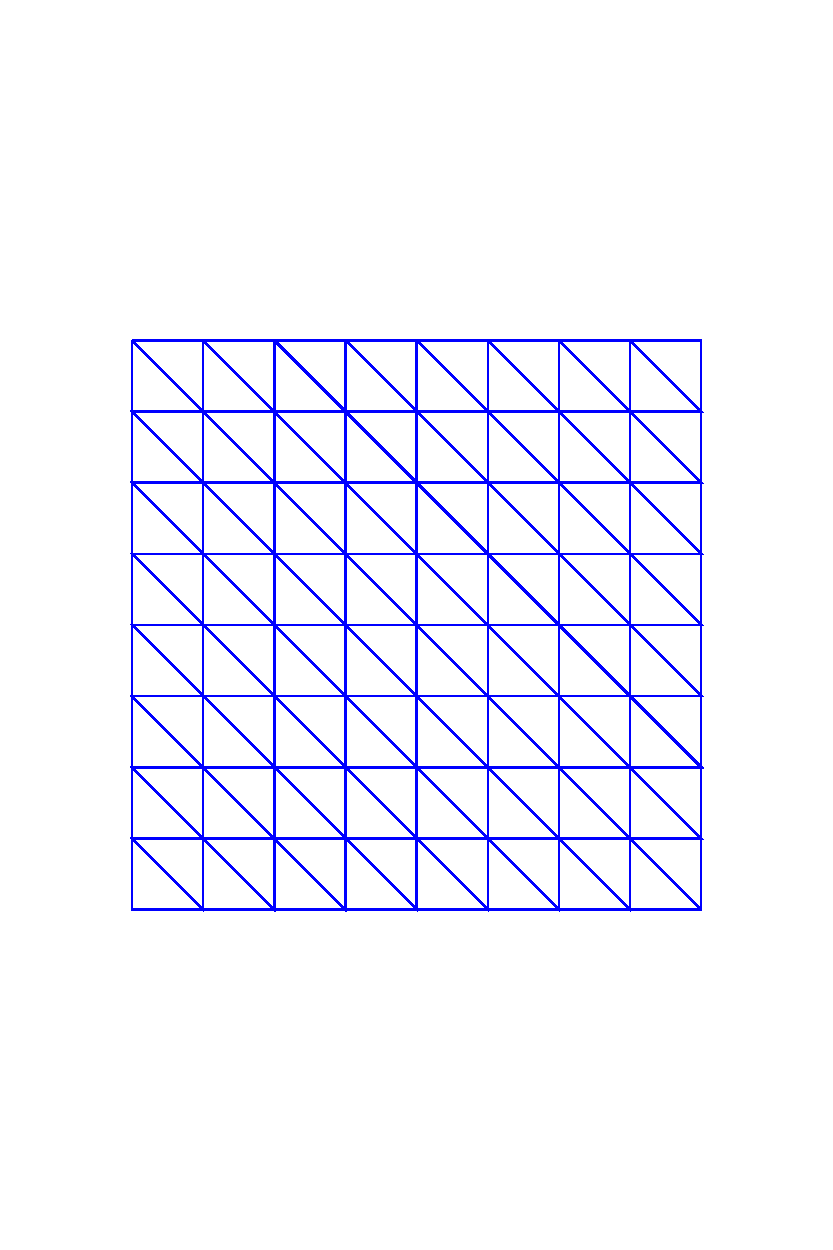
\includegraphics[scale=.5]{../Results/Figures/dolfin_plot_1}
    \caption{Level $3$ grid on unit square domain}
  \label{fig:2Dmesh}
\end{figure}
The first column of all convergence and iteration tables below will show the grid level.

\paragraph{Stopping criteria} ~\\

Recall that both the Navier-Stokes equations as well as the full MHD problem are a set of non-linear equations. Section \ref{sec:nonlinear} outlines the process in which we linearise the problem and then solve for the updates. The stopping criteria that we enforce is the following:
\begin{itemize}
  \item NS: $\|\delta {u} \|_{\mathpzc{p}}+\|\delta p \|_{\mathpzc{p}} < \mbox{tol}$,
  \item MHD: $\|\delta {u} \|_{\mathpzc{p}}+\|\delta p \|_{\mathpzc{p}}+\|\delta {b} \|_{\mathpzc{p}}+\|\delta r \|_{\mathpzc{p}} < \mbox{tol}$,
\end{itemize}
where $\mathpzc{p}=\infty$ or $2$. The tolerance is stated for each example run within this thesis.

\paragraph{Initial guess} ~\\

To start the Picard iterations given in section \ref{sec:nonlinear} we require an initial guess. To form the initial guess, we solve the decoupled Stokes problem
$$
\left(
\begin{array}{cc}
A & B^T \\
B & 0 \\
\end{array}
\right)
\left(
\begin{array}{c}
u \\
p \\
\end{array}
\right)=\left(
\begin{array}{c}
f \\
0 \\
\end{array}
\right),
$$
then the Maxwell subproblem
$$\left(
\begin{array}{cc}
M-C & D^T \\
D & 0 \\
\end{array}
\right)
\left(
\begin{array}{c}
b \\
r \\
\end{array}
\right)=\left(
\begin{array}{c}
g \\
0 \\
\end{array}
\right).$$
Here the term $C$ corresponds the the coupling term using $u$ (the initial guess for the velocity field).

When solving these two systems, the convergence tolerance which we use is important. In particular, inaccurate solutions cause problems with non-homogeneous boundary conditions. This is because if the matrix system with the boundary conditions applied is not solve to a sufficient accuracy then there will be errors in the boundary data. When we solve for the updates we enforce homogeneous Dirichlet boundary conditions (i.e. zero boundary conditions) on the velocity ($u$), magnetic ($b$) and multiplier ($r$) fields. This therefore means that if the Stokes and Maxwell solves are not done accurately enough then when solving for the updates errors will remain within the boundary conditions. Thus the errors norms for the full MHD system will be capped by the accuracy of the Stokes and Maxwell solve for the initial guess.





\section{Navier-Stokes equations}
\label{sec:NS_validation}
Before considering the full discretised MHD problem, we require that the Navier-Stokes subproblem performs as expected in terms of the error estimates and preconditioner scalability. To check the validity of the FEniCS code, we introduce two smooth test problems, the first in 2D and the second in 3D.




\subsection{2D smooth solution}

Consider the domain $\Omega =(0, 1)^2$ with boundary $\partial \Omega$. Since we are considering a purely Dirichlet problem then $\Gamma_D = \partial \Omega$ and $\Gamma_N = \emptyset$. Taking the kinematic viscosity to be $\nu = 1$, then we choose the source terms $\uu{f}$ from the analytical solution
\begin{subequations} \nonumber
\begin{eqnarray}\nonumber
\uu{u}(x,y) &=&
\begin{pmatrix}
\sin(x)\exp(x+y)+\cos(y)\exp(x+y)\\
-\sin(y)\exp(x+y)
\end{pmatrix},\\
\nonumber
p(x,y) &=& x^3\sin(y)+\exp(x+y).
\end{eqnarray}
\end{subequations}

Running the \fenics code produces the following table of results:
\begin{table}[h!] \small
\begin{center}
\begin{tabular}{cccccccc}
\hline
$l$ &    Dofs $\uu{u}_h/p_h$ & $\|\uu{u}-\uu{u}_h\|_{L^2(\Omega)}$ & order & $\|\uu{u}-\uu{u}_h\|_{H^1(\Omega)}$ & order &        $\|{p}-{p}_h\|_{L^2(\Omega)}$ & order \\
\hline
 3 &     578/81 &  2.2100e-04 &     - &  1.5645e-02 &     - &  7.2758e-03 &      - \\
 4 &    2,178/289 &  2.7598e-05 &     3.00 &  3.9133e-03 &     2.00 &  1.8190e-03 &      2.00 \\
 5 &    8,450/1,089 &  3.4465e-06 &     3.00 &  9.7822e-04 &     2.00 &  4.5025e-04 &      2.01 \\
 6 &   33,282/4,225 &  4.3072e-07 &     3.00 &  2.4455e-04 &     2.00 &  1.1341e-04 &      1.99 \\
 7 &  132,098/16,641 &  5.3836e-08 &     3.00 &  6.1137e-05 &     2.00 &  2.8639e-05 &      1.99 \\
 8 &  526,338/66,049 &  6.7291e-09 &     3.00 &  1.5284e-05 &     2.00 &  7.0146e-06 &      2.03 \\
\hline
\end{tabular}
\caption{Convergence table for 2D Navier-Stokes smooth solution - Picard tolerance 1e-10}
\label{tab:NS_2D_smooth}
\end{center}
\end{table}

\noindent For Taylor-Hood elements the expected convergence rates for the velocity field in the $L^2$ and $H^1$ integral norms are third and second order and for the pressure field the $L^2$ norm is second order. From table x\ref{tab:NS_2D_smooth} we can see that we obtain third order in $L^2$, second order FOR $H^1$ in the velocity fields and second order in $L^2$ for the pressures. This is precisely what we expect from Taylor-Hood elements.

\subsection{3D smooth solution}

The three dimensional set up is very similar as with the 2D case. This time the domain is the unit cube, i.e. $\Omega =(0, 1)^3$ with boundary $\partial \Omega$. Again the test problem has only Dirichlet boundary conditions, so that $\Gamma_D = \partial \Omega$ and $\Gamma_N = \emptyset$. As before the kinematic viscosity is $\nu = 1$, then the source term $\uu{f}$ is calculated from the analytical solution
\begin{subequations} \nonumber
\begin{eqnarray}\nonumber
\uu{u}(x,y,z) &=&
\begin{pmatrix}
-\exp(x+y+z)\sin(y) + \exp(x+y+z)\sin(z)\\
\exp(x+y+z)\sin(x) - \exp(x+y+z)\sin(z)\\
-\exp(x+y+z)\sin(x) + \exp(x+y+z)\sin(y)
\end{pmatrix}, \\
\nonumber
p(x,y,z) &=&  \exp(x+y+z) + \sin(y).
\end{eqnarray}
\end{subequations}
Running the 3D code produces table \ref{tab:NS_3D_smooth} which shows the errors and convergence rates.
\begin{table}[h!] \small
\begin{center}
    \begin{tabular}{cccccccc}
    \hline
    $l$ &    Dofs $\uu{u}_h/p_h$ & $\|\uu{u}-\uu{u}_h\|_{L^2(\Omega)}$ & order & $\|\uu{u}-\uu{u}_h\|_{H^1(\Omega)}$ & order &        $\|{p}-{p}_h\|_{L^2(\Omega)}$ & order \\
    \hline
    1 &    375/27 &  2.6211e-02 &     - &  4.5804e-01 &     - &  1.7725e+00 &      - \\
    2 &   2,187/125 &  3.2997e-03 &     2.99 &  1.1547e-01 &     1.99 &  2.8602e-01 &      2.63 \\
    3 &   14,739/729 &  4.1267e-04 &     3.00 &  2.8944e-02 &     2.00 &  4.0587e-02 &      2.82 \\
    4 &  107,811/4,913 &  5.1565e-05 &     3.00 &  7.2416e-03 &     2.00 &  6.4794e-03 &      2.65 \\
    5 &  823,875/35,937 &  6.4443e-06 &     3.00 &  1.8108e-03 &     2.00 &  1.2724e-03 &      2.35 \\
    \hline
    \end{tabular}
\caption{Convergence table for 3D Navier-Stokes smooth solution - Picard tolerance 1e-5}
\label{tab:NS_3D_smooth}
\end{center}
\end{table}

\noindent From the table we can see that the convergence rates are the same as the 2D test solution in the previous section for the velocity field. However, we see that for the pressure field we get a slightly higher than expected order, namely about 2.5. We have seen this trend for multiple different examples that have been run but never have we seen an order lower than 2.

\subsection{Least Squares Commutator}

Section \ref{sec:NSprecond} outlines the two main preconditioning techniques for the Navier-Stokes equations. In order to have a scalable preconditioner for the full MHD system we need to check the performance of both LSC and PCD for our Navier-Stokes subproblem.

First considered the LSC preconditioner. Recall that to apply the LSC preconditioner we need to apply
\begin{equation} \label{eq:NS_precond_results}
  \left(
\begin{array}{cc}
F & B^T \\
0 & M_{S}
\end{array}
\right)^{-1}
\end{equation}
where
$$M_{S} = (B Q^{-1} B^T)(BQ^{-1}FQ^{-1}B^T)^{-1}(B Q^{-1} B^T)$$
at each GMRES iteration. This amounts to solving systems associated with $F$ and $B Q^{-1} B^T$, which has been outlined in section \ref{sec:NSprecond}. We do this by using a direct solve for $F$ and approximate $B Q^{-1} B^T \approx B \, \mbox{diag}(Q)^{-1} B^T$ then use a direct solve. Since $B \, \mbox{diag}(Q)^{-1} B^T$ is singular (the constant vector is in the null space) then we apply a small shift to the diagonal to ensure the invertability for the direct solver. Using GMRES with a relative tolerance stopping criteria of 1e-5 produces table \ref{tab:LSC_2D} of iteration results.
\begin{table}[h!] \small
\begin{center}
    \begin{tabular}{cccccc}
    \hline
    l &    Dofs &  \multicolumn{4}{ c }{Average iterations}\\
     & $\uu{u}_h/p_h$ & $\nu=10$ &  $\nu=1$ &  $\nu=0.1$&  $\nu=0.01$ \\
    \hline
     1 &      50/9 &     5 &     5 &    6 &    8 \\
     2 &     162/25 &    10 &    10 &   10 &   21 \\
     3 &     578/81 &    16 &    16 &   15 &   30 \\
     4 &    2,178/289 &    25 &    24 &   24 &   31 \\
     5 &    8,450/1,089 &    48 &    47 &   46 &   39 \\
     6 &   33,282/4,225 &   103 &    86 &   77 &   63 \\
     7 &  132,098/16,641 &   190 &   190 &  141 &  131 \\
    \hline
    \end{tabular}
\caption{Iteration table for LSC preconditioner  for 2D example -  Picard tolerance 1e-10}
\label{tab:LSC_2D}
\end{center}
\end{table}

Table \ref{tab:LSC_2D} shows that as the grid level increases the number of iterations GMRES takes to converge to the set tolerance increases. This is a relatively unknown problem when using Taylor-Hood elements. This therefore requires us to consider using PCD as the Navier-Stokes subproblem preconditioner instead.



\subsection{Pressure Convection-Diffusion}

As for LSC an application of \eqref{eq:NS_precond_results} is applied at each GMRES iteration. However, for PCD the Schur complement approximation $M_S$ is given by:
$$M_S = A_p F_p^{-1}W.$$
Instead of applying the  PCD preconditioner exactly (direct solves) we will use approximate solves. We therefore use a single multigrid V-cycle to approximately solve both $F$ and $A_p$ and Conjugate Gradient (CG) \cite{hestenes1952methods} with a block Jacobi preconditioner and outer tolerance of 1e-5 for $W$. With the outer tolerance of GMRES the same as before we obtain the tables of iterations for both the 2D and 3D examples.

\subsubsection{2D example}
Running the 2D example gives table \ref{tab:PCD_2D}.
\begin{table}[h!] \small
\begin{center}
    \begin{tabular}{cccccc}
    \hline
    l &    Dofs &  \multicolumn{4}{ c }{Average iterations}\\
     & $\uu{u}_h/p_h$ & $\nu=10$ &  $\nu=1$ &  $\nu=0.1$&  $\nu=0.01$ \\
    \hline
      5 &     8450/1089 &    17 &  15 &  18 &  5053 \\
      6 &    33,282/4,225 &    18 &  15 &  18 &   144 \\
      7 &   132,098/16,641 &    18 &  15 &  18 &    41 \\
      8 &   526,338/66,049 &    18 &  15 &  18 &    40 \\
      9 &  2,101,250/263,169 &    18 &  15 &  18 &    40 \\
    \hline
    \end{tabular}
\caption{Iteration table for PCD preconditioner  for 2D example -  Picard tolerance 1e-10}
\label{tab:PCD_2D}
\end{center}
\end{table}

\noindent From table \ref{tab:PCD_2D} we can see that as the mesh level increases then the iteration numbers stay roughly constant. This is what we expect and require for the Navier-Stokes subproblem preconditioner. Also, the table shows iteration number for multiple different values of the kinematic viscosity $\nu$. Again as expected, as the viscosity decreases (i.e. the equations become more convection dominated) the iterations increase.



%%%%%%%%%%%%%%%%%%%%%%%%%%%%%%%%%%%%%%%%%%%%%%%%%%%%%%%%%%%%%%%%%%%%%%%%%%%%%%%%%%%%%%%%%%%%%%%%%%%%%%%%%%%%%%%%%%%%%%%%%%%%%%%%%%%%%%%%%%%%%%%%%%%%%%%%%%%%%%%%%%%%%%%%%%%%%%%%%%%%%%%%%%%%%%%%%%%%%%%%%%%%%%%%%%%%%%%%%%%%%%%%%%%%%%%%%%%%%%%%%%%%%%%%%%%%%%%%%%%%%%%%%%%%%%%%%%%%%%%%%%%%%%%%%%%%%%%%%%%%%%%%%%%%%%%%%%%%%%%%%%%%%%%%%%%%%%%%%%%%%%%%%%%%%%%%%%%%%%%%%%%%%%%%%%%%%%%%%%%%%%%%%%%%%%%%%%%%%%%%%%%%%%%%%%%%%%%%%%%%%%%%%%%%%%%%%%%%%%%%%%%%%%%%%%%%%%%%%%%%%%%%%%%%%%%%%%%%%%%%%%%%%%%%%%%%%%%%%%%%%%%%%%%%%%%%%%%%%%%%%%%%%%%%%%%%%%%%%%%%%%%%%%%%%%%%%%%%%%%%%%%%%%%%%%%%%%%%%%%%%%%%%%%%%%%%%%%%%%%%%%%%%%%%%%%%%%%%%%%%%%%%%%%%%%%%%%%%%%%%%%%%%%%%%%%%%%%%%%%%%%%%%%%%%%%%%%%%%%%%%%%%%%%%%%%%%%%%%%%%%%%%%%%%%%%
\subsubsection{3D example}

Running the 3D code produces the following table.
\begin{table}[h!] \small
\begin{center}
    \begin{tabular}{cccccc}
    \hline
    l &    Dofs &  \multicolumn{4}{ c }{Average iterations}\\
     & $\uu{u}_h/p_h$ & $\nu=10$ &  $\nu=1$ &  $\nu=0.1$&  $\nu=0.01$ \\
    \hline

    \hline
    \end{tabular}
\caption{Iteration table for PCD preconditioner  for 3D example -  Picard tolerance 1e-10}
\label{tab:PCD_3D}
\end{center}
\end{table}

%%%%%%%%%%%%%%%%%%%%%%%%%%%%%%%%%%%%%%%%%%%%%%%%%%%%%%%%%%%%%%%%%%%%%%%%%%%%%%%%%%%%%%%%%%%%%%%%%%%%%%%%%%%%%%%%%%%%%%%%%%%%%%%%%%%%%%%%%%%%%%%%%%%%%%%%%%%%%%%%%%%%%%%%%%%%%%%%%%%%%%%%%%%%%%%%%%%%%%%%%%%%%%%%%%%%%%%%%%%%%%%%%%%%%%%%%%%%%%%%%%%%%%%%%%%%%%%%%%%%%%%%%%%%%%%%%%%%%%%%%%%%%%%%%%%%%%%%%%%%%%%%%%%%%%%%%%%%%%%%%%%%%%%%%%%%%%%%%%%%%%%%%%%%%%%%%%%%%%%%%%%%%%%%%%%%%%%%%%%%%%%%%%%%%%%%%%%%%%%%%%%%%%%%%%%%%%%%%%%%%%%%%%%%%%%%%%%%%%%%%%%%%%%%%%%%%%%%%%%%%%%%%%%%%%%%%%%%%%%%%%%%%%%%%%%%%%%%%%%%%%%%%%%%%%%%%%%%%%%%%%%%%%%%%%%%%%%%%%%%%%%%%%%%%%%%%%%%%%%%%%%%%%%%%%%%%%%%%%%%%%%%%%%%%%%%%%%%%%%%%%%%%%%%%%%%%%%%%%%%%%%%%%%%%%%%%%%%%%%%%%%%%%%%%%%%%%%%%%%%%%%%%%%%%%%%%%%%%%%%%%%%%%%%%%%%%%%%%%%%%%%%%%%%%%%

\section{Maxwell's equations}
\label{sec:Maxwell_validation}

As for the Navier-Stokes subproblem (section \ref{sec:NS_validation}), we consider a 2D and 3D test solution to validated the \fenics code for the Maxwell subproblem.

\subsection{2D smooth solution}
\label{sec:2D_maxwell}
Again, consider the domain $\Omega =(0, 1)^2$ with boundary $\partial \Omega$. Since we are considering a purely Dirichlet problem then $\Gamma_D = \partial \Omega$ and $\Gamma_N = \emptyset$. Now choose the source terms $\uu{g}$ that satisfy the analytical solution
\begin{subequations} \nonumber
\begin{eqnarray}\nonumber
\uu{b}(x,y) &=&
\begin{pmatrix}
\exp(x + y)\cos(x)\\
\exp(x + y)\sin(x) - \exp(x + y)\cos(x)
\end{pmatrix},\\
\nonumber
r(x,y) &=& \sin(2\pi x)\sin(2\pi y).
\end{eqnarray}
\end{subequations}

\begin{table}[h!] \small
\begin{center}
\begin{tabular}{cccccc}
\hline
l &    Dofs $\uu{b}_h/r_h$ & $\|\uu{b}-\uu{b}_h\|_{L^2(\Omega)}$ & order & $\|\uu{b}-\uu{b}_h\|_{H(curl,\Omega)}$ & order \\
\hline
1 &      48/25 &  9.3833e-02 &    - &  1.0696e-01 &       - \\
2 &     176/81 &  2.3350e-02 &    2.01 &  2.7088e-02 &       1.98 \\
3 &     672/289 &  5.8372e-03 &    2.00 &  6.4220e-03 &       2.08 \\
4 &    2,624/1,089 &  1.4597e-03 &    2.00 &  1.4586e-03 &       2.14 \\
5 &   10,368/4,225 &  3.6497e-04 &    2.00 &  3.5066e-04 &       2.06 \\
6 &   41,216/16,641 &  9.1246e-05 &    2.00 &  8.6688e-05 &       2.02 \\
7 &  164,352/66,049 &  2.2812e-05 &    2.00 &  2.1609e-05 &       2.00 \\
\hline
\end{tabular}
\caption{Convergence table for 2D Maxwell smooth solution - Magnetic field}
\label{tab:2D_maxwell_magnetic}
\end{center}
\end{table}
\begin{table}[h!] \small
\begin{center}
\begin{tabular}{cccccc}
\hline
l &    Dofs $\uu{b}_h/r_h$ & $\|{r}-{r}_h\|_{L^2(\Omega)}$ & order & $\|{r}-{r}_h\|_{H^1(\Omega)}$ & order\\
\hline
 1 &      48/25 &  2.7761e-01 &    - &  2.8932e+00 &     - \\
 2 &     176/81 &  4.3540e-02 &    2.67 &  9.3299e-01 &     1.63 \\
 3 &     672/289 &  4.8633e-03 &    3.16 &  2.5904e-01 &     1.85 \\
 4 &    2,624/1,089 &  5.6724e-04 &    3.10 &  6.6810e-02 &     1.96 \\
 5 &   10,368/4,225 &  6.9363e-05 &    3.03 &  1.6841e-02 &     1.99 \\
 6 &   41,216/16,641 &  8.6203e-06 &    3.01 &  4.2193e-03 &     2.00 \\
 7 &  164,352/66,049 &  1.0760e-06 &    3.00 &  1.0554e-03 &     2.00 \\

\hline
\end{tabular}
\caption{Convergence table for 2D Maxwell smooth solution - multiplier field}
\label{tab:2D_maxwell_multiplier}

\end{center}
\end{table}

For Maxwell equations we use second order \nedelec elements  of the first kind \cite{nedelec1980mixed} and polynomial elements of the same order for the magnetic and multiplier fields respectively. Therefore, we exact second order convergence in $\|\uu{b}-\uu{b}_h\|_{L^2(\Omega)}$, $\|\uu{b}-\uu{b}_h\|_{H(curl,\Omega)}$ and $\|{r}-{r}_h\|_{H^1(\Omega)}$ and third order in $\|{r}-{r}_h\|_{L^2(\Omega)}$. Tables \ref{tab:2D_maxwell_magnetic} and \ref{tab:2D_maxwell_multiplier} show that we do obtain the expected rates of convergence for both the magnetic and multiplier fields.


\subsection{3D smooth solution}

As for the 3D Navier-Stokes problem the domain is the unit cube, i.e. $\Omega =(0, 1)^3$ with boundary $\partial \Omega$. Again the test problem has only Dirichlet boundary conditions then $\Gamma_D = \partial \Omega$ and $\Gamma_N = \emptyset$. Using the anayltical solution
\begin{subequations} \nonumber
\begin{eqnarray}\nonumber
\uu{b}(x,y,z) &=&
\begin{pmatrix}
-\exp(x + y + z)\sin(y) + \exp(x + y + z)\sin(z)\\
\exp(x + y + z)\sin(x) - \exp(x + y + z)\sin(z)\\
-\exp(x + y + z)\sin(x) + \exp(x + y + z)\sin(y)
\end{pmatrix},\\
\nonumber
r(x,y,z) &=& \sin(2\pi x)\sin(2\pi y)\sin(2\pi z),
\end{eqnarray}
 the source term $\uu{g}$ is defined.
\end{subequations}
\begin{table}[h!] \small
\begin{center}
    \begin{tabular}{cccccc}
    \hline
l &    Dofs $\uu{b}_h/r_h$ & $\|\uu{b}-\uu{b}_h\|_{L^2(\Omega)}$ & order & $\|\uu{b}-\uu{b}_h\|_{H(curl,\Omega)}$ & order \\
    \hline
 1 &     436/125 &  5.3312e-02 &    0.00 &  3.5258e-01 &       0.00 \\
 2 &    2,936/729 &  1.4192e-02 &    1.91 &  8.9944e-02 &       1.97 \\
 3 &   21,424/4,913 &  3.5801e-03 &    1.99 &  2.2690e-02 &       1.99 \\
 4 &  163,424/35,937 &  8.9697e-04 &    2.00 &  5.7585e-03 &       1.98 \\
    \hline
    \end{tabular}
\caption{Convergence table for 3D Maxwell smooth solution - magnetic field}
\label{tab:3D_maxwell_magnetic}
\end{center}
\end{table}

\begin{table}[h!] \small
\begin{center}
    \begin{tabular}{cccccc}
    \hline
l &    Dofs $\uu{b}_h/r_h$ & $\|{r}-{r}_h\|_{L^2(\Omega)}$ & order & $\|{r}-{r}_h\|_{H^1(\Omega)}$ & order\\
    \hline
 1 &     436/125 &  2.2689e-01 &    0.00 &  2.8923e+00 &     0.00 \\
 2 &    2,936/729 &  5.9452e-02 &    1.93 &  1.1782e+00 &     1.30 \\
 3 &   21,424/4,913 &  6.9068e-03 &    3.11 &  3.3901e-01 &     1.80 \\
 4 &  163,424/35,937 &  7.5913e-04 &    3.19 &  9.0082e-02 &     1.91 \\

    \hline
    \end{tabular}
\caption{Convergence table for 3D Maxwell smooth solution - multiplier field}
\label{tab:3D_maxwell_multiplier}
\end{center}
\end{table}


Tables \ref{tab:3D_maxwell_magnetic} and \ref{tab:3D_maxwell_multiplier} show the same orders of convergence as in the 2D case from section \ref{sec:2D_maxwell}.




\subsection{Preconditioning}

Section \ref{sec:MaxwellPrecond} introduces the preconditioning strategy that will be employed in this thesis. Recall that the preconditioner is:
\begin{equation} \nonumber
\mathcal{M}_{\rm MX} =
\begin{pmatrix}
N& 0 \\
0 & L
\end{pmatrix},
\end{equation}
where $N = M+X$ as defined in chapters \ref{sec:discretization} and  \ref{chap:precond}.  It is possible to form a scalable (i.e. iteration count stays the same as $l$ increase) application of $\mathcal{M}_{\rm MX}^{-1}$  using the algebraic multigrid method described in \cite{hiptmair2007nodal} for $N$ and standard multigrid for $L$. This, however, is very complex to implement and hence application of $\mathcal{M}_{\rm MX}^{-1}$ will be done with direct solves for the numerical results in this section.

\subsubsection{2D example}

Table \ref{tab:Maxwell_2D} shows the performance of using the preconditioner $\mathcal{M}_{\rm MX}$  with a MINRES tolerance of $1e-6$.
\begin{table}[h!] \small
\begin{center}
  \begin{tabular}{cccccc}
  \hline
   l &     Dofs $\uu{b}_h/r_h$ &  \multicolumn{4}{ c }{Number of iterations} \\
    &                 &  $\nu_m=10$ &  $\nu_m=100 $&  $\nu_m=1000 $&  $\nu_m=10000$ \\
  \hline
   5 &    10,368/4,225 &   5 &    4 &     6 &      6 \\
   6 &    41,216/16,641 &   5 &    6 &     6 &      6 \\
   7 &   164,352/66,049 &   5 &    6 &     6 &      6 \\
   8 &   656,384/263,169 &   5 &    6 &     6 &      8 \\
   9 &  2,623,488/1,050,625 &   4 &    6 &     6 &      8 \\
   10 &  10,489,856/4,198,401 &   4 &    6 &     8 &     10 \\

  \hline
\end{tabular}
\caption{Iteration table for Maxwell preconditioner  for 2D example - direct application of preconditioner}
\label{tab:Maxwell_2D}
\end{center}
\end{table}

From table \ref{tab:Maxwell_2D} we can see that as the number of MINRES iterations stays about constant as the mesh level, $l$, increases. Note that as the magnetic viscosity ($\nu_m$) increases then the number of iterations remains roughly the same.

\subsubsection{3D example}

Table \ref{tab:Maxwell_3D} presents the iteration numbers when using  $\mathcal{M}_{\rm MX}$ as the preconditioner to MINRES with tolerance $1e-6$.
\begin{table}[h!] \small
\begin{center}
\begin{tabular}{cccccc}
\hline
  l &     Dofs $\uu{b}_h/r_h$ &  \multicolumn{4}{ c }{Number of iterations} \\
    &                  &  $\nu_m=10$ &  $\nu_m=100 $&  $\nu_m=1000 $&  $\nu_m=10000$ \\
    \hline
  2 &    2,936/729 &   4 &    4 &     6 &      5 \\
  3 &   21,424/49,13 &   4 &    4 &     6 &      5 \\
  4 &  163,424/35,937 &   4 &    6 &     6 &      5 \\
\hline
\end{tabular}
\caption{Iteration table for Maxwell preconditioner  for 3D example - direct application of preconditioner}
\label{tab:Maxwell_3D}
\end{center}
\end{table}
Again, as with the 2D example we see that the number of iterations remains about constant with increasing mesh level and value of $\nu_m$.


\section{MHD problem}

Sections \ref{sec:NS_validation} and \ref{sec:Maxwell_validation} shows results for the Navier-Stokes and Maxwells equations in isolation. The next step is to incorporate these two subproblems  into the full MHD system.

\subsection{2D smooth solution}

To validate the code, we consider the following $2D$ test problem. For this problem, let the domain be the unit square $\Omega = (0, 1)^2$ with purely Dirichlet boundary conditions on $\partial \Omega$. Let $\nu = \kappa =1$, $\nu_m=\rm{1e4}$ then the source terms $\uu{f}$ and $\uu{g}$ are defined from the analytical solution:
\begin{align*} \nonumber
\uu{u}(x,y)& =\begin{pmatrix}
xy\exp(x + y) + x\exp(x + y)\\
-xy\exp(x + y) - y\exp(x + y)
\end{pmatrix},\\
p(x,y)& =\exp(y)\sin(x),\\[0.1cm]
\uu{b}(x,y)& =\begin{pmatrix}
 \exp(x + y)\cos(x) \\
 \exp(x + y)\sin(x) - \exp(x + y)\cos(x)
\end{pmatrix},\\
 r(x,y)& =x\sin(2\pi x)\sin(2\pi y).
\end{align*}

The asymptotic rates of convergence are given in tables \ref{tab:MHD_2D_smooth_fluids} to \ref{tab:MHD_2D_smooth_multiplier}.
\begin{table}[h!] \small
\begin{center}
\begin{tabular}{cccccccc}
\hline
$l$ &    Dofs $\uu{u}_h/p_h$ & $\|\uu{u}-\uu{u}_h\|_{L^2(\Omega)}$ & order & $\|\uu{u}-\uu{u}_h\|_{H^1(\Omega)}$ & order &        $\|{p}-{p}_h\|_{L^2(\Omega)}$ & order \\
\hline
 1 &      50/9 &  8.1347e-02 &     0.00 &  1.2748e+00 &     0.00 &  2.8866e-01 &      0.00 \\
 2 &     162/25 &  1.0566e-02 &     2.94 &  3.3018e-01 &     1.95 &  3.7372e-02 &      2.95 \\
 3 &     578/81 &  1.3354e-03 &     2.98 &  8.3246e-02 &     1.99 &  4.8723e-03 &      2.94 \\
 4 &    2,178/289 &  1.6744e-04 &     3.00 &  2.0840e-02 &     2.00 &  7.2809e-04 &      2.74 \\
 5 &    8,450/1,089 &  2.0998e-05 &     3.00 &  5.2110e-03 &     2.00 &  1.5307e-04 &      2.25 \\
 6 &   33,282/4,225 &  2.6528e-06 &     2.98 &  1.3028e-03 &     2.00 &  3.7059e-05 &      2.05 \\
 7 &  132,098/16,641 &  3.4518e-07 &     2.94 &  3.2570e-04 &     2.00 &  9.2136e-06 &      2.01 \\
 8 &  526,338/66,049 &  4.9471e-08 &     2.80 &  8.1425e-05 &     2.00 &  2.3009e-06 &      2.00 \\

\hline
\end{tabular}
\caption{Convergence table for 2D MHD smooth solution - Picard tolerance 1e-8}
\label{tab:MHD_2D_smooth_fluids}
\end{center}
\end{table}


\begin{table}[h!] \small
\begin{center}
\begin{tabular}{cccccc}
\hline
l &    Dofs $\uu{b}_h/r_h$ & $\|\uu{b}-\uu{b}_h\|_{L^2(\Omega)}$ & order & $\|\uu{b}-\uu{b}_h\|_{H(curl,\Omega)}$ & order \\
\hline
 1 &      48/25 &  1.1206e-01 &     0.00 &  1.7807e-01 &        0.00 \\
 2 &     176/81 &  2.8439e-02 &     1.98 &  4.5429e-02 &        1.97 \\
 3 &     672/289 &  7.1388e-03 &     1.99 &  1.1414e-02 &        1.99 \\
 4 &    2,624/1,089 &  1.7867e-03 &     2.00 &  2.8571e-03 &        2.00 \\
 5 &   103,68/4,225 &  4.4679e-04 &     2.00 &  7.1450e-04 &        2.00 \\
 6 &   41,216/16,641 &  1.1171e-04 &     2.00 &  1.7864e-04 &        2.00 \\
 7 &  164,352/66,049 &  2.7927e-05 &     2.00 &  4.4661e-05 &        2.00 \\
 8 &  656,384/263,169 &  6.9818e-06 &     2.00 &  1.1165e-05 &        2.00 \\
\hline
\end{tabular}
\caption{Convergence table for 2D MHD smooth solution - Magnetic field}
\label{tab:MHD_2D_smooth_magnetic}
\end{center}
\end{table}



\begin{table}[h!] \small
\begin{center}
\begin{tabular}{cccccc}
\hline
l &    Dofs $\uu{b}_h/r_h$ & $\|{r}-{r}_h\|_{L^2(\Omega)}$ & order & $\|{r}-{r}_h\|_{H^1(\Omega)}$ & order\\
\hline
 1 &      48/25  &  1.8438e-01 &     0.00 &  1.9449e+00 &     0.00 \\
 2 &     176/81  &  2.8307e-02 &     2.70 &  6.0694e-01 &     1.68 \\
 3 &     672/289  &  3.1214e-03 &     3.18 &  1.6510e-01 &     1.88 \\
 4 &    2,624/1,089  &  3.6035e-04 &     3.11 &  4.2417e-02 &     1.96 \\
 5 &   103,68/4,225  &  4.3890e-05 &     3.04 &  1.0683e-02 &     1.99 \\
 6 &   41,216/16,641  &  5.4485e-06 &     3.01 &  2.6757e-03 &     2.00 \\
 7 &  164,352/66,049  &  6.7988e-07 &     3.00 &  6.6923e-04 &     2.00 \\
 8 &  656,384/263,169  &  8.4948e-08 &     3.00 &  1.6733e-04 &     2.00 \\
\hline
\end{tabular}
\caption{Convergence table for 2D MDH smooth solution - multiplier field}
\label{tab:MHD_2D_smooth_multiplier}
\end{center}
\end{table}

The results shown in tables \ref{tab:MHD_2D_smooth_fluids} to \ref{tab:MHD_2D_smooth_multiplier} agree with the optimal rates for $\|\uu{u}-\uu{u}_h\|_{L^2(\Omega)}$, $\|\uu{u}-\uu{u}_h\|_{H^1(\Omega)}$, $\|\uu{b}-\uu{b}_h\|_{L^2(\Omega)}$, $\|\uu{b}-\uu{b}_h\|_{H(curl,\Omega)}$, $\|{r}-{r}_h\|_{L^2(\Omega)}$ and $\|{r}-{r}_h\|_{H^1(\Omega)}$. The pressure field  exhibits a little higher than expected rate of convergence for $l<5$ but settles down to second order for the higher levels.



% ======================================
%                3D
% ======================================


\subsection{3D smooth solution}

As for the 3 dimensional examples we consider a test problem discretised on a unit cube domain with Dirichlet boundary conditions. Let $\nu = \kappa =1$, $\nu_m=\rm{1e4}$ and the analytical solution as:
\begin{align*} \nonumber
\uu{u}(x,y,z)& =\begin{pmatrix}
-xy\exp(x + y + z) + xz\exp(x + y + z))\\
xy\exp(x + y + z) - yz\exp(x + y + z)\\
-xz\exp(x + y + z) + yz\exp(x + y + z)
\end{pmatrix},\\
p(x,y,z)& =\exp(x + y + z)\sin(y),\\[0.1cm]
\uu{b}(x,y,z)& =\begin{pmatrix}
 -\exp(x + y + z)\sin(y) + \exp(x + y + z)\sin(z) \\
xy\exp(x + y + z) - yz\exp(x + y + z) \\
-\exp(x + y + z)\sin(x) + \exp(x + y + z)\sin(y)
\end{pmatrix},\\
 r(x,y,z)& =\sin(2\pi x)\sin(2\pi y)\sin(2\pi z),
\end{align*}
then the source terms $\uu{f}$ and $\uu{g}$ are defined.

\begin{table}[h!] \small
\begin{center}
\begin{tabular}{cccccccc}
\hline
$l$ &    Dofs $\uu{u}_h/p_h$ & $\|\uu{u}-\uu{u}_h\|_{L^2(\Omega)}$ & order & $\|\uu{u}-\uu{u}_h\|_{H^1(\Omega)}$ & order &        $\|{p}-{p}_h\|_{L^2(\Omega)}$ & order \\
\hline
  1 &     375/27 &  4.2196e-03 &     - &  7.8282e-02 &     - &  5.0614e-02 &      - \\
  2 &    2187/125 &  5.2733e-04 &     3.00 &  1.9495e-02 &     2.01 &  9.0306e-03 &      2.49 \\

 3 &   14739/729 &  6.5749e-05 &     3.00 &  4.8664e-03 &     2.00 &  1.9035e-03 &      2.25 \\

 4 &  107811/4913 &  8.2092e-06 &     3.00 &  1.2161e-03 &     2.00 &  4.5311e-04 &      2.07 \\

\hline
\end{tabular}
\caption{Convergence table for 3D MHD smooth solution - Picard tolerance 1e-8}
\label{tab:MHD_3D_smooth_fluids}
\end{center}
\end{table}


\begin{table}[h!] \small
\begin{center}
\begin{tabular}{cccccc}
\hline
l &    Dofs $\uu{b}_h/r_h$ & $\|\uu{b}-\uu{b}_h\|_{L^2(\Omega)}$ & order & $\|\uu{b}-\uu{b}_h\|_{H(curl,\Omega)}$ & order \\
\hline
1 &     436/125 &  3.9931e-03 &     - &  2.4817e-02 &        - \\
2 &    2936/729 &  1.1211e-03 &     1.83 &  7.4101e-03 &        1.74 \\
3 &   21424/4913 &  2.9642e-04 &     1.92 &  1.9439e-03 &        1.93 \\
4 &  163424/35937 &  7.5494e-05 &     1.97 &  4.9180e-04 &        1.98 \\
\hline
\end{tabular}
\caption{Convergence table for 3D MHD smooth solution - Magnetic field}
\label{tab:MHD_3D_smooth_magnetic}
\end{center}
\end{table}



\begin{table}[h!] \small
\begin{center}
\begin{tabular}{cccccc}
\hline
l &    Dofs $\uu{b}_h/r_h$ & $\|{r}-{r}_h\|_{L^2(\Omega)}$ & order & $\|{r}-{r}_h\|_{H^1(\Omega)}$ & order\\
\hline
 1 &     436/125 &       7.4750e-04 &     - &  1.0113e-02 &     - \\
 2 &    2936/729 &      9.2457e-05 &     3.02 &  2.9368e-03 &     1.78 \\
 3 &   21424/4913 &         1.1182e-05 &     3.05 &  7.7197e-04 &     1.93 \\
 4 &  163424/35937 &       1.3829e-06 &     3.02 &  1.9597e-04 &     1.98 \\
\hline
\end{tabular}
\caption{Convergence table for 3D MDH smooth solution - multiplier field}
\label{tab:MHD_3D_smooth_multiplier}
\end{center}
\end{table}

From tables \ref{tab:MHD_3D_smooth_fluids} to \ref{tab:MHD_3D_smooth_multiplier} it can be seen that we obtain the same convergence orders as with the $2D$ case.


\subsection{Parameter decoupling tests}
\label{sec:ParaTest}

There are two different decoupling schemes considered in thesis. These effectiveness of these approaches is likely to be limited by the parameter set up of the problem, i.e. the fluid viscosity ($\nu$), magnetic viscosity ($\nu_m$) and the coupling number ($\kappa$). In this section we will look at how these three schemes perform when fixing two parameters and varying the second. We will only look at varying $\kappa$ and $\nu$ since $\nu_m$ appears within all three schemes. In the tables we denote (P) as the full MHD system given in \cref{eq:picard}, (MD) is the magnetic decoupling scheme \cref{eq:picard_explicit_MD} and (CD) is complete decoupling \cref{eq:picard_explicit_CD}. Also, if the Picard iterations do not converge then this is denoted by - in the table.

\subsubsection{Viscosity test}

The first test we will consider is to vary the fluid viscosity results are represented in table \ref{tab:MHD_2D_viscosity_decouple_test}. The parameter set up here is that the non-linear Picard tolerance is $1e-5$, coupling number $\kappa = 1$ and magnetic viscosity $\nu_m = 10$.

{\setlength{\tabcolsep}{.2em} \begin{table}[h!] \small
\begin{center}
\begin{tabular}{|cc|ccc|ccc|ccc|ccc|}
\hline
  \multicolumn{2}{|c }{} &  \multicolumn{3}{|c| }{$\nu=1$} &  \multicolumn{3}{|c| }{$\nu=0.1$} &  \multicolumn{3}{|c| }{$\nu=0.01$}&     \multicolumn{3}{|c| }{$\nu=0.001$} \\
l &     DoF &  (P) &  (MD) &  (CD) &  (P) &  (MD) &  (CD)  &   (P) &  (MD) &  (CD) &   (P) &  (MD) &  (CD)    \\
\hline
 3 &     1,620 &   5 &   7 &  15 &  8 &  10 &  - &  12 &  14 & -  &  40 &  40 & -  \\
 4 &     6,180 &   5 &   7 &  15 &  8 &  10 &  - &  12 &  14 &  - &  40 &  40 &  - \\
 5 &    24,132 &   5 &   7 &  15 &  8 &  10 & -  &  12 &  14 &   -&  19 &  19 & -  \\
 6 &    95,364 &   5 &   7 &  15 &  8 &  10 &  - &  12 &  14 &  - &  17 &  19 & -  \\
 7 &   379,140 &   5 &   7 &  15 &  8 &  10 &  - &  12 &  14 &   -&  17 &  19 &  - \\
 8 &  1,511,940 &   5 &   7 &  15 &  8 &  10 &  - &  12 &  14 & -  &  17 &  19 & -  \\
\hline
\end{tabular}
\caption{Number of non-linear iterations for various values of $\nu$. Let the Picard tolerance to be $1e-5$, $\kappa = 1$ and $\nu_m = 10$.}
\label{tab:MHD_2D_viscosity_decouple_test}
\end{center}
\end{table}}
As the fluid viscosity ($\nu$) decreases then the equations that determine the fluid flow become more convection dominated. Thus we would expect that the complete decoupling scheme might break down for small $\nu$ as for this decoupling scheme we remove the convection term. This is precisely what we what we see from the results in table \ref{tab:MHD_2D_viscosity_decouple_test}. However, the full MHD problem and magnetic decoupling cases perform very similarly in terms of the number of Picard iterations it takes to converge to the solution for $\kappa = 1$. For $\nu = 0.0001$ all schemes break down and do not converge. This maybe due to the stability of the convection discretisation.


\subsubsection{Coupling number test}

The other parameter test that we exam is to vary the coupling term.
{\setlength{\tabcolsep}{.15em} \begin{table}[h!] \small
\begin{center}
\begin{tabular}{|cc|ccc|ccc|ccc|ccc|ccc|}
\hline
  \multicolumn{2}{|c }{} &  \multicolumn{3}{ |c| }{$\kappa=0.1$} &  \multicolumn{3}{|c| }{$\kappa=1$} &  \multicolumn{3}{|c| }{$\kappa=10$}&     \multicolumn{3}{|c| }{$\kappa=100$}&     \multicolumn{3}{|c| }{$\kappa=1000$} \\
l &     DoF &  (P) &  (MD) &  (CD) &  (P) &  (MD) &  (CD)  &   (P) &  (MD) &  (CD) &   (P) &  (MD) &  (CD)  &   (P) &  (MD) &  (CD)    \\
\hline
3 &    1,620 &  5 &  5 &  13 &   5 &   5 &  13 &   6 &   7 &  17 &    7 &   13 &   26 &     7 &    93 &     - \\
4 &    6,180 &  5 &  5 &  13 &   5 &   5 &  15 &   6 &   7 &  18 &    7 &   13 &   26 &     7 &    93 &     - \\
5 &   24,132 &  5 &  5 &  13 &   5 &   5 &  15 &   6 &   7 &  18 &    7 &   13 &   26 &     7 &    93 &     - \\
6 &   95,364 &  5 &  5 &  14 &   5 &   5 &  15 &   6 &   7 &  18 &    7 &   13 &   26 &     7 &    93 &     - \\
7 &  379,140 &  5 &  5 &  14 &   5 &   5 &  15 &   6 &   7 &  18 &    7 &   13 &   26 &     7 &    93 &     - \\
8 &  1,511,940 &  5 &  5 &  14 &   5 &   5 &  15 &   6 &   7 &  18 &    7 &   13 &   26 &     7 &    93 &     - \\
\hline
\end{tabular}
\caption{Number of non-linear iterations for various values of $\nu_m$. LLet the Picard tolerance to be $1e-5$, $\nu = 1$ and $\nu_m = 1e2$.}
\label{tab:MHD_2D_kappa_decouple_test}
\end{center}
\end{table}}
This test shows how increasing the coupling term effects the number of non-linear iterations for each of the three schemes. We expect that the full Picard (P) scheme would perform best with both the magnetic and complete decoupling schemes breaking down as $\kappa$ increases. Table \ref{tab:MHD_2D_kappa_decouple_test} shows that this is what happens. Notice that the complete decoupling scheme completely breaks down for $\kappa > 100$ whereas the number of non-linear iterations for magnetic decoupling stays roughly constant for each mesh level but is larger than for the full Picard iterations.

\section{Preconditioned MHD problem}

% In section \ref{sec:ParaTest} we have performed a parameter test to see how the decoupling techiques performed with respect to the parameters $\kappa$ and $\nu$. From tables \ref{tab:MHD_2D_viscosity_decouple_test} and \ref{tab:MHD_2D_kappa_decouple_test} it is possible to see that the decoupling schemes perform

Sections \ref{sec:MHDprecond} and \ref{sec:MDprecond} introduced the three preconditioning techniques that will be applied to each of the decoupling schemes and the full MHD system. In this section we will look at the performances of these strategies with respect to time and iteration count for various tolerances.


\subsection{MHD problem}

Recall form section \ref{sec:MHDprecond} that the preconditioner for the full MHD problem ${\mathcal K}_{\rm MH}$ given in \eqref{eq:mhd_saddle} is
\begin{equation} \nonumber
\mathcal{M}_{\rm MH} =
\left(
\begin{array}{cccc}
F & B^T & C^T & 0\\
0 & -S & 0 & 0 \\
-C & 0 & N & 0\\
0 & 0 & 0 & L
\end{array}
\right),
\end{equation}
where $S$ will be the PCD approximation to the Schur complement of the Navier-Stokes subproblem. To apply $\mathcal{M}_{\rm MH}$ as the preconditioner we employ an inner Krylov solver where the preconditioner is the same as  $\mathcal{M}_{\rm MH}$ but importantly we drop the coupling terms, i.e.
\begin{equation} \nonumber
\mathcal{M}_{\rm innerMH} =
\left(
\begin{array}{cccc}
F & B^T & 0 & 0\\
0 & -S & 0 & 0 \\
0 & 0 & N & 0\\
0 & 0 & 0 & L
\end{array}
\right).
\end{equation}
There are four solves ($F$, $S$, $N$ and $L$) to apply $\mathcal{M}_{\rm innerMH}$ as an inner preconditioner. Each will be a direct solve apart from the PCD approximation in which apply $S^{-1} = W^{-1}F_p A_p^{-1}$ where $W^{-1}$ and $A_p^{-1}$ will be direct solves as well.

\subsection{Magnetic decoupling}
\begin{table}[h!] \small
\begin{center}
\begin{tabular}{cccccc}
\hline
 l &     DoF &  Soln Time &  picard iterations &  NS iters &  M iters \\
\hline
 3 &    1620 &   0.039161 &                  8 &        52 &        3 \\
 4 &    6180 &   0.097946 &                  8 &        48 &        3 \\
 5 &   24132 &   0.447303 &                  8 &        52 &        3 \\
 6 &   95364 &   2.109198 &                  8 &        52 &        3 \\
 7 &  379140 &   9.697754 &                  8 &        50 &        3 \\
 8 &  1511940 &  46.675882                  &8&        51&        3 \\
 9&  6038532&  539.038188&                  8&        51&        3 \\
\hline
\end{tabular}
\caption{$tol = 1e-5    kappa = 1.0/2 Mu_m =1e2 MU = 0.1$}
\end{center}
\end{table}

\subsection{Complete decoupling}

\begin{table}[h!] \small
\begin{center}
\begin{tabular}{ccccccc}
\hline
 l &      DoF &  AV solve Time &  Total picard time &  picard iterations & Av NS iters & Av M iters \\
\hline
 3 &     1620 &          0.030 &               0.32 &                  5 &        29.4 &        2.6 \\
 4 &     6180 &          0.072 &               0.72 &                  5 &        29.4 &        2.6 \\
 5 &    24132 &          0.290 &               2.36 &                  5 &        29.0 &        2.8 \\
 6 &    95364 &          1.552 &              11.14 &                  5 &        29.0 &        2.8 \\
 7 &   379140 &          7.164 &              48.96 &                  5 &        29.0 &        2.8 \\
 8 &  1511940 &         36.180 &             232.27 &                  5 &        29.0 &        2.8 \\
 9 &  6038532 &        159.17 &            1618.24 &                  5 &        29.0 &        2.8 \\
\hline
\end{tabular}
\caption{$tol = 1e-5    kappa = 1.0/2 Mu_m =1e2 MU = 10$}
\end{center}
\end{table}